\subsection{Datasets}

\begin{table}
    \centering
    \begin{tabular}{ccccc}
        \toprule
        Dataset & Nodes & Edges & Classes & Features \\
        \midrule
        CiteSeer & 3,327 & 9,228 & 6 & 3,703 \\ 
        Amazon\_Photos & 7,650 & 238,163 & 8 & 745 \\
        Cora & 19,793 & 126,842 & 70 & 8,710 \\
        PubMed & 19,717 & 88,651 & 3 & 500 \\
        Coauthor\_CS &  18,333 & 163,788 & 15 & 6,805 \\
        Coauthor\_Physics & 34,493 & 495,924 & 5 & 8,415 \\
        \bottomrule
    \end{tabular}
    \caption{Summary statistics for Datasets chosen for evaluation.}
    \label{tab:conformal:datasets}
\end{table}


We selected datasets of varying sizes to evaluate the performance of the graph conformal prediction methods.
For the citation datasets, the nodes are publications, and the edges denote citation relationships.
Features are bag-of-words representations of the documents.
The task is to predict the category of each publication.
\textbf{CiteSeer} is a citation network dataset designed for the node classification task, with nodes as publications and edges denoting citation relationships.
\textbf{Amazon\_Photos} is a segment of the Amazon co-purchase graph~\cite{mcauley2015image} where nodes represent goods, edges represent goods frequently bought together, features are bag-of-words representations of product reviews, and the task is to predict the category of each good.
\textbf{Cora} We use CoraFull~\cite{shchur2018pitfalls}, an extended version of the common Cora citation network dataset.
Summary statistics for the datasets are provided in Table~\ref{tab:conformal:datasets}.
The objective is to predict the category of each node (publication).
\textbf{PubMed} is a citation network dataset designed for the node classification task, with nodes as publications and edges denoting citation relationships. The goal is to predict the category of each node (publication).
For all chosen datasets, we used the version provided by the Deep Graph Library~\cite{wang2019dgl}.
\textbf{Coauthor\_CS} and \textbf{Coauthor\_Physics} are co-authorship graphs extracted from the Microsoft Academic Graph and used for KDD Cup 2016. In this dataset, nodes are authors and edges denoting co-authorship relationships. The task is to predict the most active field of study for each author.

To help characterize the behavior of different approaches, we categorize these into sizes based on the number of nodes, with \textbf{Cora} and \textbf{Amazon\_Photos} designated as small (S), \textbf{CiteSeer}, \textbf{PubMed}, and \textbf{Coauthor\_CS} as medium (M), and \textbf{Coauthor\_Physics} as large (L).

\subsection{Metrics}
We evaluate the following metrics for the graph conformal prediction methods:
\begin{itemize}
    \item \textbf{Coverage:} The proportion of test instances for which the true label is contained in the prediction set.
    \item \textbf{Efficiency:} The average size of the prediction set.
    \item \textbf{Label Stratified Coverage:} The mean of coverage for each class. This metric is useful for understanding whether a method is adaptive and has balanced coverage for different classes.
    \item \textbf{Size Stratified Coverage:} The mean of coverage across different sizes of prediction sets. This metric is useful for understanding whether a method is adaptive and does not under/over cover hard/easy samples.
    %\item \textbf{Size Stratified Coverage Violation:} Measures the maximum deviation from the coverage goal across different prediction set sizes. 
    %\item \textbf{Singleton Hit Ratio:} The proportion of test instances for which the true label is the only label in the prediction set. This metric measures the frequency with which a method does not require generation of a prediction set having multiple labels.
\end{itemize}

\subsection{Methods}
We discussed the theoretical and empirical tradeoffs of different methods in Section~\ref{chp:graphConformal:sec:conformal_scores_tradeoffs}.
For completeness, we list all the methods that we compare here.
\textbf{Threshold Prediction Sets}~\cite{sadinle2019least}, with two variants, TPS and TPS-Classwise (using class wise thresholds for adapting to class imbalance).
\textbf{Adaptive Prediction Sets}~\cite{romano2020classification} with two variants, APS and APS-Randomized (using the uniform random quantile adjustments).
\textbf{Regularized Adaptive Prediction Sets}~\cite{angelopoulos2021uncertainty}, a variation of APS with a regularization term to ensure that the prediction sets are not too large.
\textbf{Diffused Adaptive Prediction Sets}~\cite{zargarbashi23conformal}, with two variations DAPS and DTPS, which uses a diffusion process over TPS-Classwise.
\textbf{Normalized Adaptive Prediction Sets}~\cite{clarkson2023distribution} with three variations corresponding to the weighing function used.
\textbf{CF-GNN}~\cite{huang2024uncertainty}, a GNN based approach for conformal prediction. We label the original implementation of CFGNN as CFGNN-Original and our improved implementations as CFGNN-APS (using randomized APS as the loss function for training/evaluation) and CFGNN-TPS (using TPS as the loss function for training/evaluation).

%\subsection{Notes on Parameter Tuning and Evaluation}
%\pmcomment{TODO for final version}

\section{Results}


\begin{figure}
    \centering
    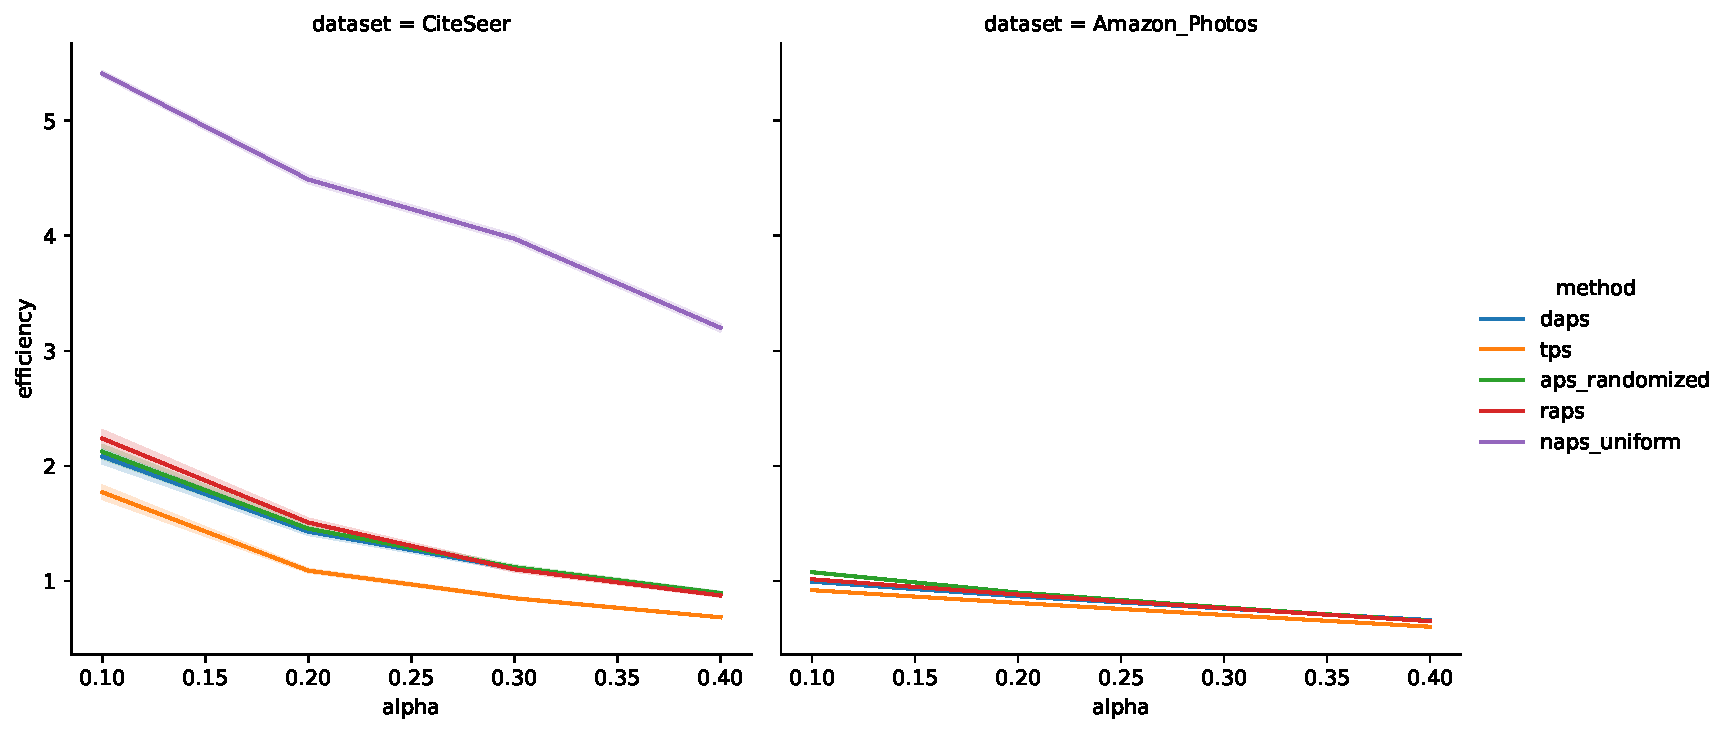
\includegraphics[width=\linewidth]{graphConformal/figures/split/small_datasets_efficiency.pdf}
    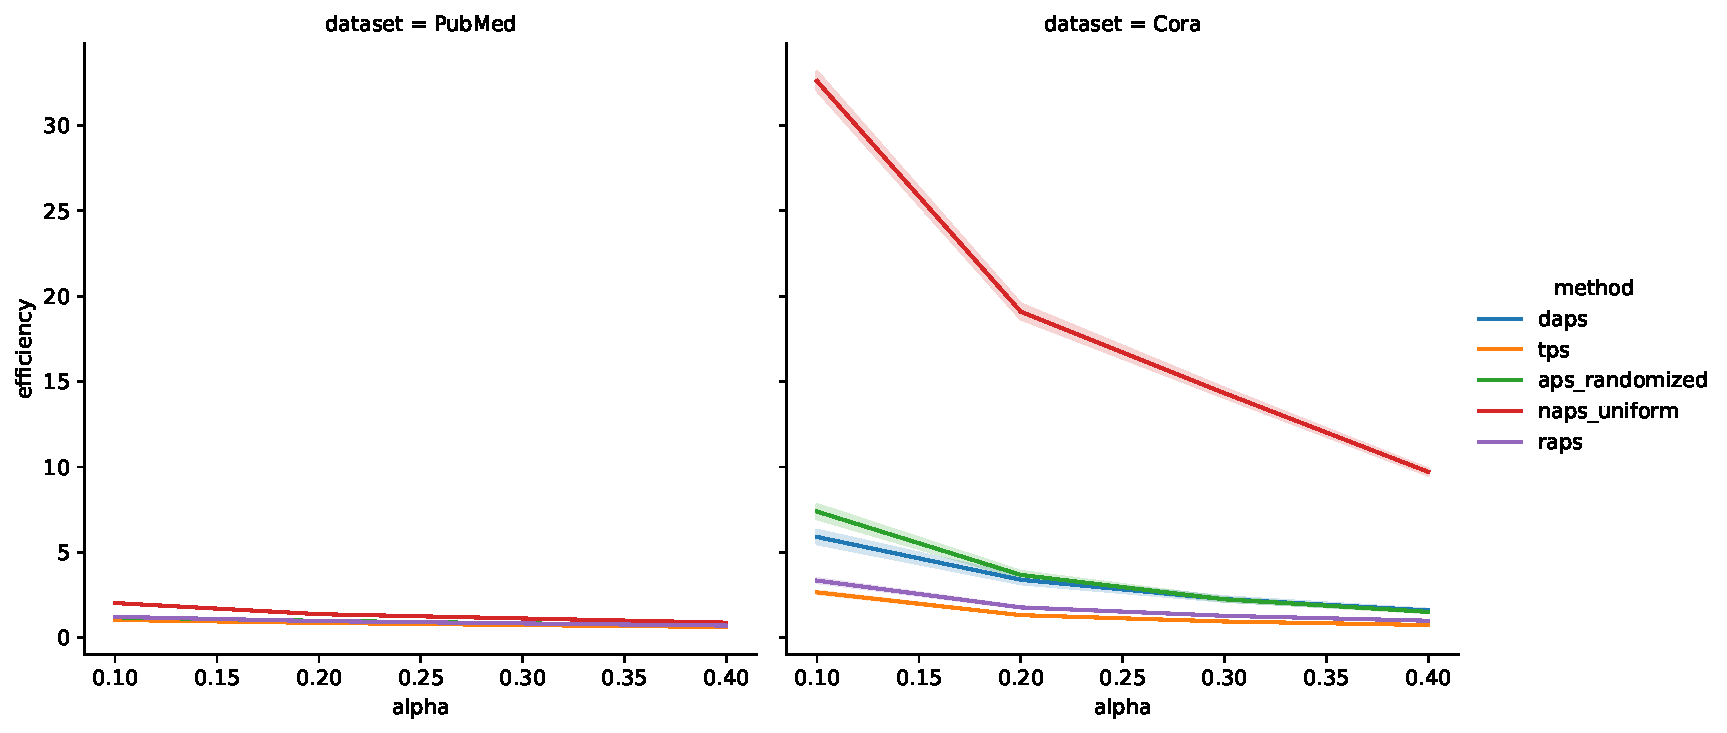
\includegraphics[width=\linewidth]{graphConformal/figures/split/med_1_datasets_efficiency.pdf}
    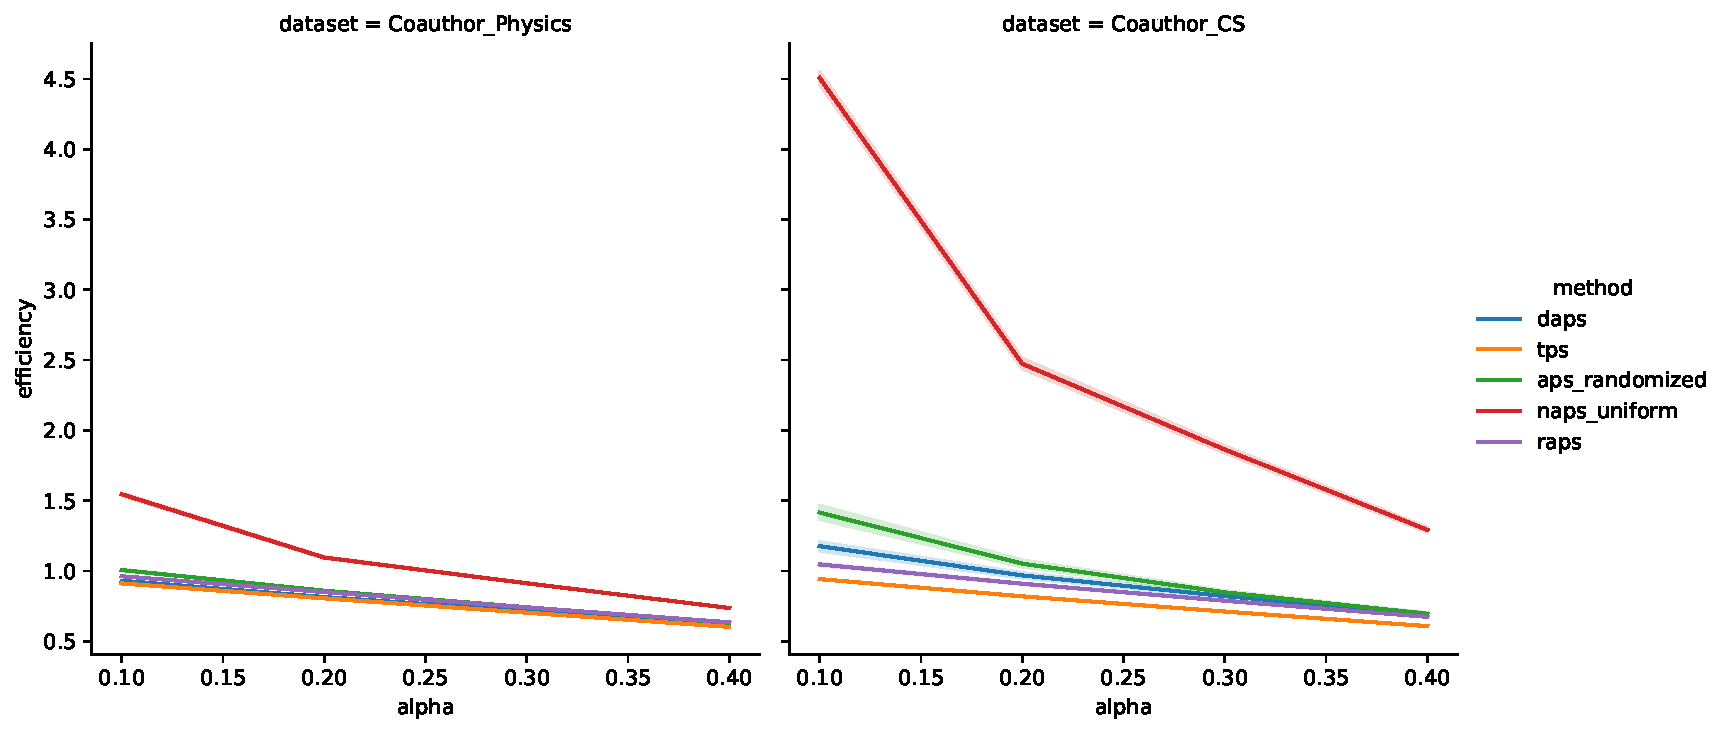
\includegraphics[width=\linewidth]{graphConformal/figures/split/med_2_datasets_efficiency.pdf}
    \caption{Plots for efficiency vs $\alpha$ for the major methods across the all the datasets. Among the baseline methods, TPS consistently has the best efficiency. Result for FS paritttion}
    \label{fig:fs:conformal:efficiency_vs_alpha}
\end{figure}

First, we analyze the efficiency of the methods across different datasets.
Figure~\ref{fig:fs:conformal:efficiency_vs_alpha} shows the efficiency of the methods across different datasets.
We find that for each dataset, irrespective of the train/validation/calib split, TPS is consistently the most efficient method.
However, this often comes at a cost to adaptability.
In the next set of results, we show how using classwise thresholds can provide some degree of adaptability for TPS.
Next, we focus on the adaptability provided by using classwise TPS.

\subsection{Adaptability through Classwise TPS}
\begin{figure}
    \centering
    \begin{subfigure}{0.48\linewidth}
    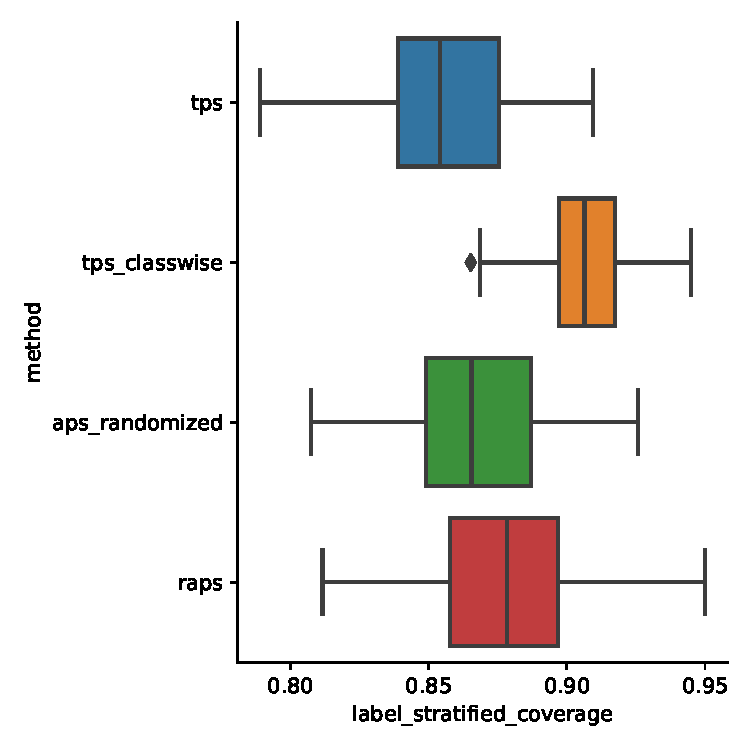
\includegraphics[width=\linewidth]{graphConformal/figures/split/citeseer_label_stratified_coverage}
    \end{subfigure}
    \begin{subfigure}{0.48\linewidth}
        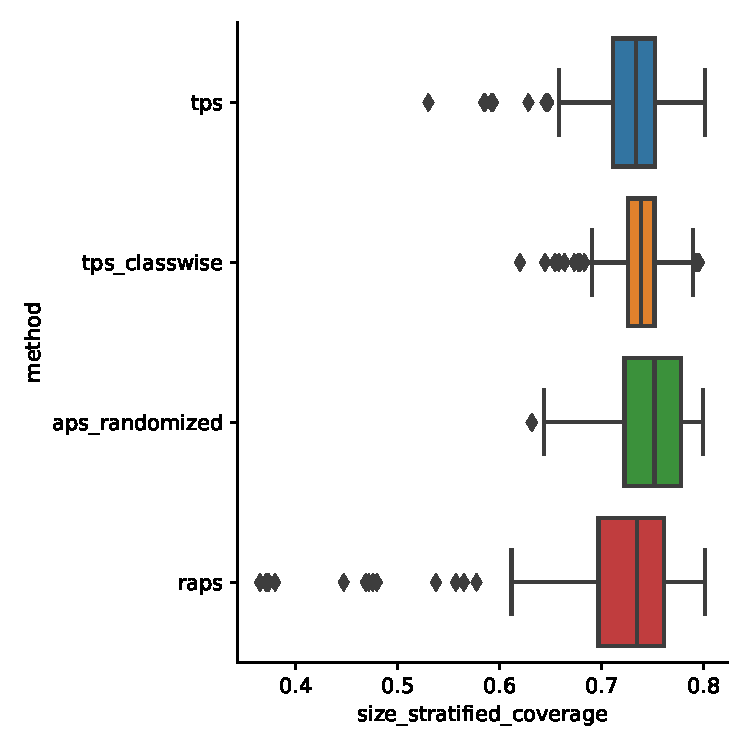
\includegraphics[width=\linewidth]{graphConformal/figures/split/citeseer_size_stratified_coverage} 
     \end{subfigure}

    \begin{subfigure}{0.48\linewidth}
    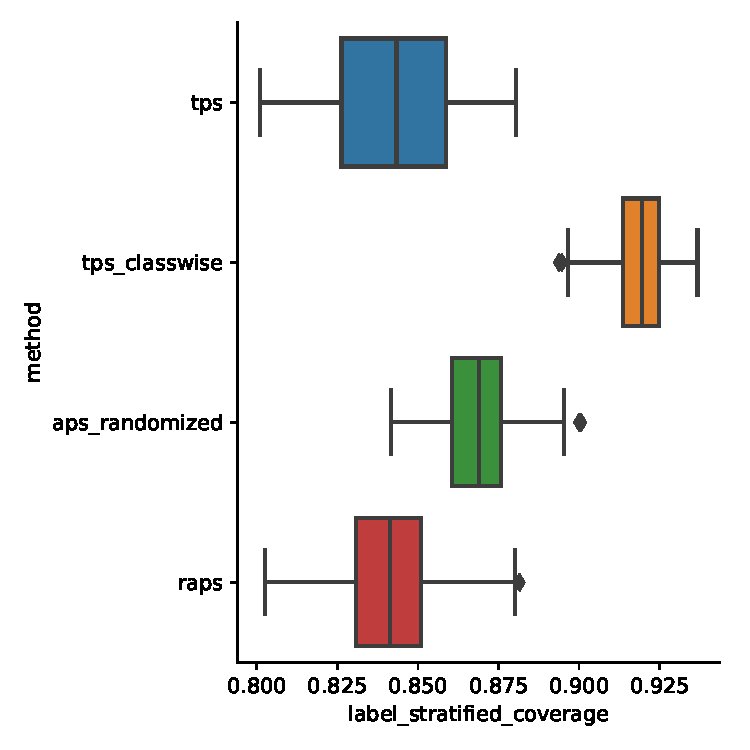
\includegraphics[width=\linewidth]{graphConformal/figures/split/cora_label_stratified_coverage}
    \end{subfigure}
    \begin{subfigure}{0.48\linewidth}
        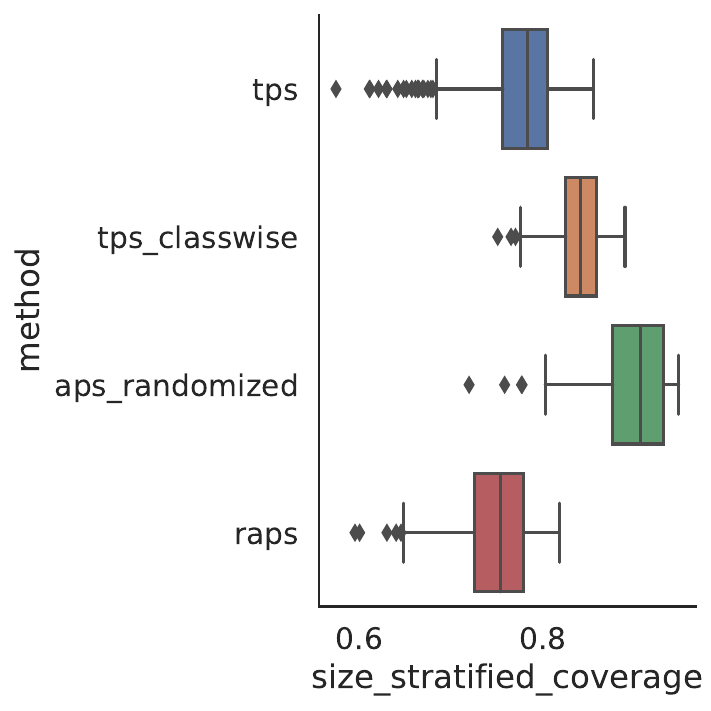
\includegraphics[width=\linewidth]{graphConformal/figures/split/cora_size_stratified_coverage} 
     \end{subfigure}
     \caption{At a target $\alpha = 0.1$. Boxplots indicating (left) Label Stratified Coverage. (right) Size Stratified Coverage for CiteSeer (top) and Cora(bottom). Classwise TPS provides adaptability when stratified by labels without sacrificing size stratified coverage. Results for FS splits.}
     \label{fig:fs:conformal:citeseer_adaptability}
\end{figure}
From Figure~\ref*{fig:fs:conformal:citeseer_adaptability}, we see that using classwise TPS successfully provides stratified coverage over different labels without sacrificing size stratified coverage vs a baseline TPS.
At the limit, even when reducing the number of samples per class from Figure~\ref{fig:nspc:citeseer:ssc}, we can see that the loss in size stratified coverage is minimal.
Thus, at least for the datasets we studied, TTPS-Classwise is a good candidate for an adaptive version of TPS.
\begin{figure}
    \begin{subfigure}{0.48\linewidth}
        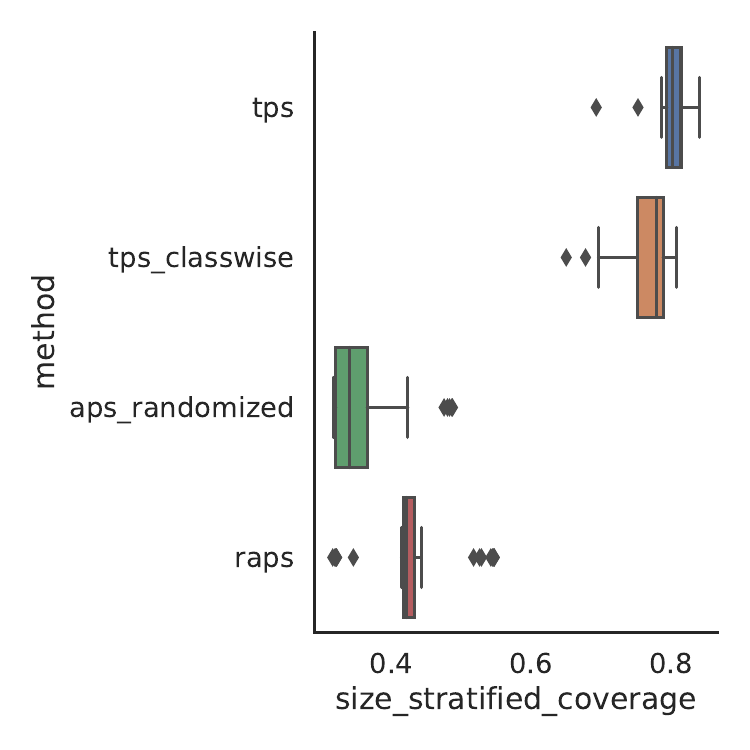
\includegraphics[width=\linewidth]{graphConformal/figures/nspc/citeseer_nspc_10_size_stratified_coverage}
    \end{subfigure}
    \begin{subfigure}{0.48\linewidth}
        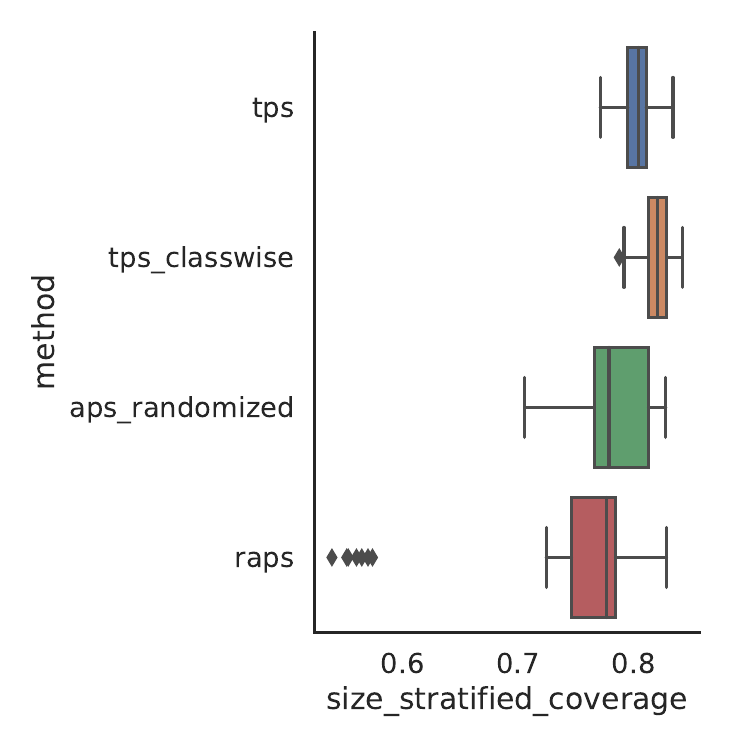
\includegraphics[width=\linewidth]{graphConformal/figures/nspc/citeseer_nspc_20_size_stratified_coverage}
    \end{subfigure}
    \caption{At a target $\alpha = 0.1$, boxplots for size stratified coverage with calibration sets having (left) 10 samples per class and (right) 20 samples per class for CiteSeer.}
    \label{fig:nspc:citeseer:ssc}
\end{figure}

\subsection{APS Randomized Sets}
\begin{figure}
    \centering
    \begin{subfigure}{0.8\linewidth}
    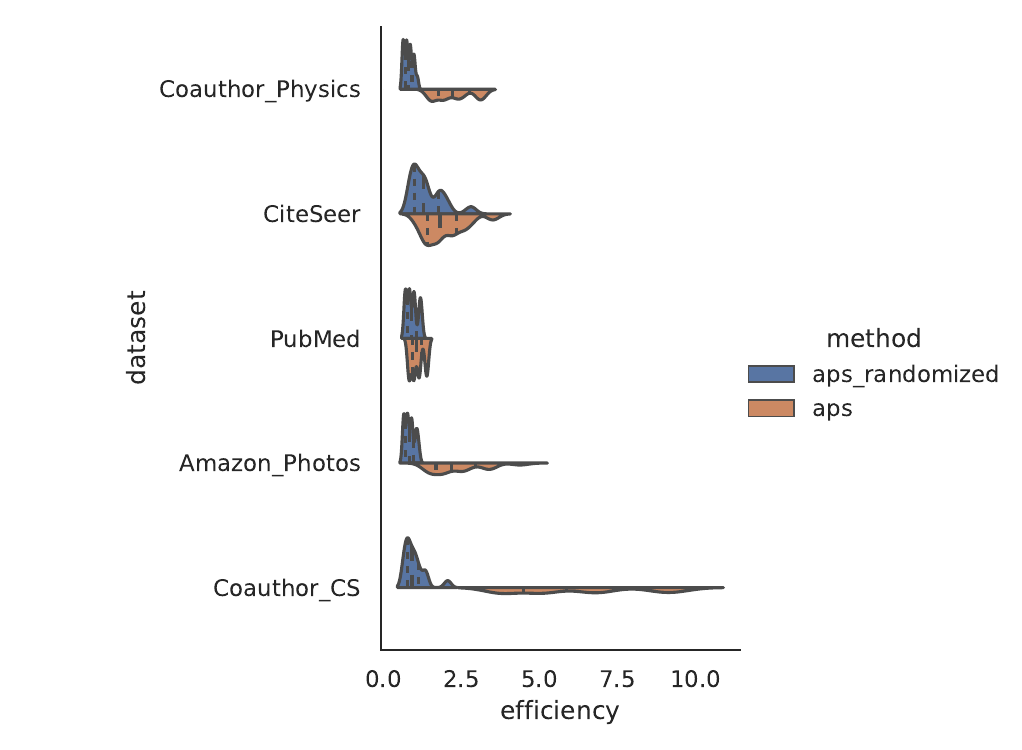
\includegraphics[width=\linewidth]{graphConformal/figures/split/aps_randomized_efficiency}
    \end{subfigure}
    \begin{subfigure}{0.6\linewidth}
        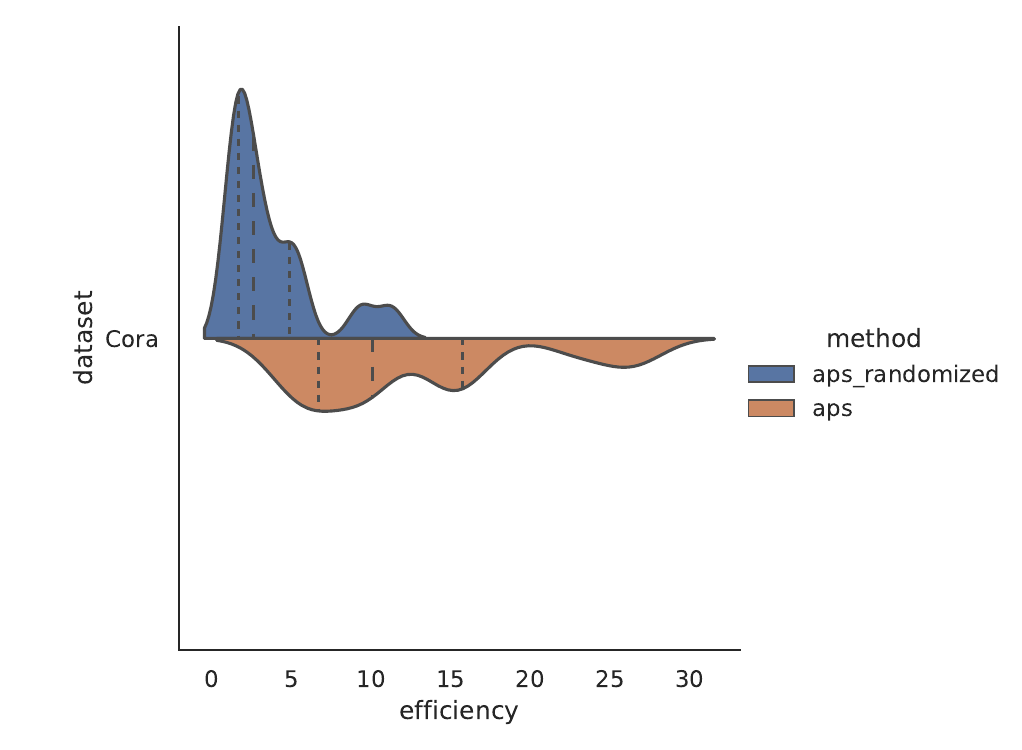
\includegraphics[width=\linewidth]{graphConformal/figures/split/aps_randomized_efficiency_cora}
    \end{subfigure}
    \caption{Violin plots denoting efficiencies of APS and Randomized APS across different datasets and multiple runs in FS split. Randomization consistently improves over the non-randomized version.}
    \label{fig:fs:conformal:aps_vs_randomized}
\end{figure}

\begin{figure}
    \centering
    \begin{subfigure}{0.8\linewidth}
    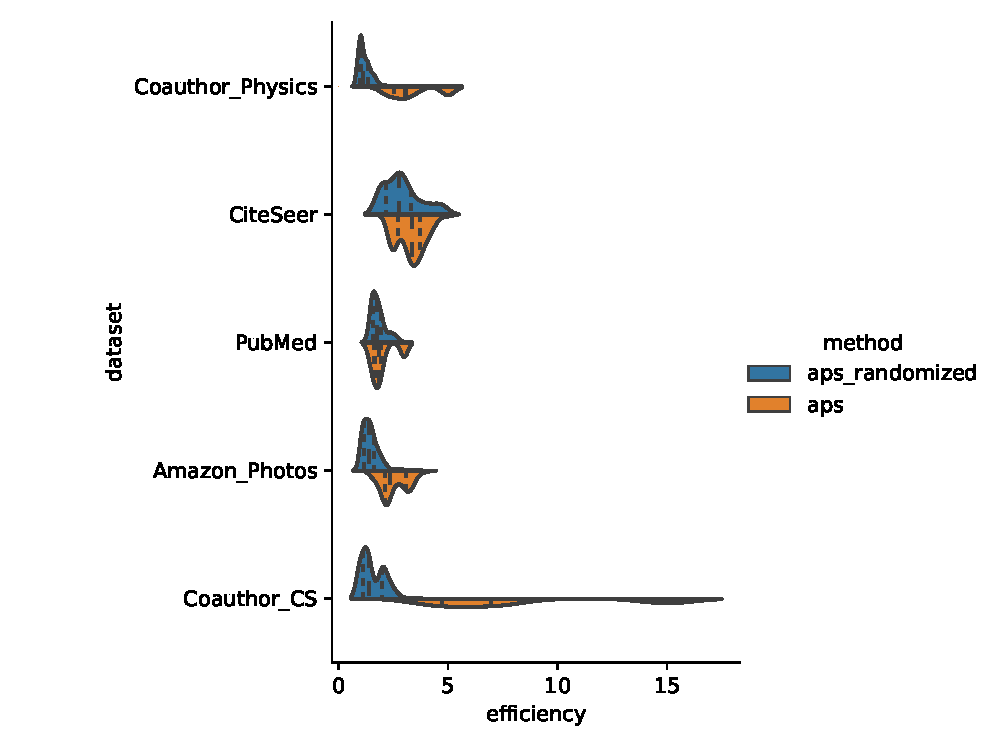
\includegraphics[width=\linewidth]{graphConformal/figures/nspc/aps_randomized_efficiency}
    \end{subfigure}
    \begin{subfigure}{0.6\linewidth}
        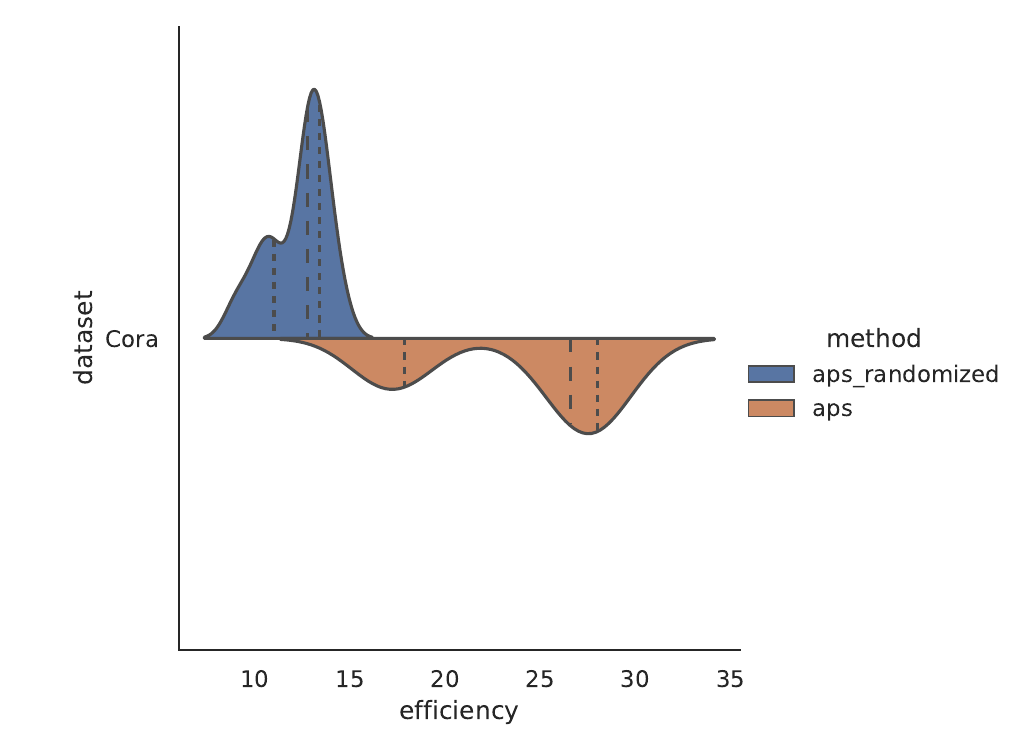
\includegraphics[width=\linewidth]{graphConformal/figures/nspc/aps_randomized_efficiency_cora}
    \end{subfigure}
    \caption{Violin plots denoting efficiencies of APS and Randomized APS across different datasets and multiple runs in LC split. Randomization consistently improves over the non-randomized version.}
    \label{fig:nspc:conformal:aps_vs_randomized}
\end{figure}
Figure~\ref{fig:fs:conformal:aps_vs_randomized} and Figure~\ref{fig:nspc:conformal:aps_vs_randomized} provide violin plots that compare tehe efficiency of randomized and non-randomized version of APS across different datasets and $\alpha$.
We observe that in each case, the peaks associated with the randomized version lie to the left of those associated with the non-randomized version.
This indicates that the randomized version consistently provides a more efficient prediction set.
This effect is most pronounced for a dataset having a large number of potential classes (Cora), which matches with the intuition from Theorem~\ref{them:APS:efficiency} - with a $(K-1)\left(\alpha_c^{A} - \alpha_C^{\Tilde{A}}\right)$ term contributing to the improved efficiency and least pronounced for PubMed, which has the smallest $K=3$.
Overall, the empirical results show that the effect of randomized APS is more apparent for larger number of classes $K$.
% \pmcomment{Show that TPS-classwise does not sacrifice much on efficiency either}

\subsection{Diffusion Thresholded Adaptatiive Sets}
\begin{figure}
    \centering
    \begin{subfigure}{0.7\linewidth}
        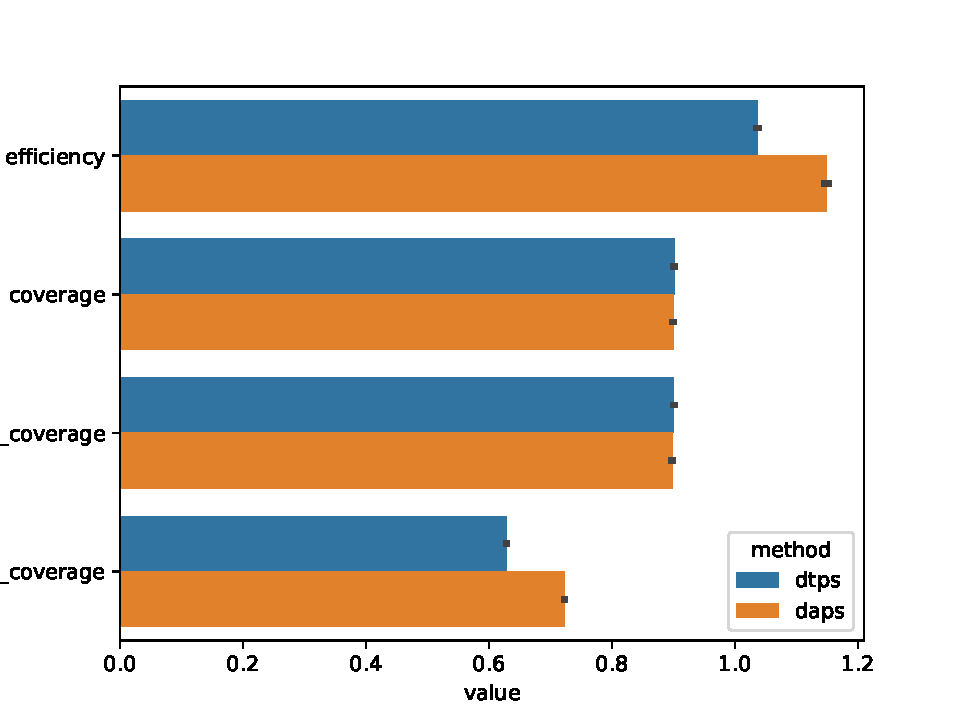
\includegraphics[width=\linewidth]{graphConformal/figures/split/daps_dtps_pubmed}
    \end{subfigure}
    \begin{subfigure}{0.7\linewidth}
        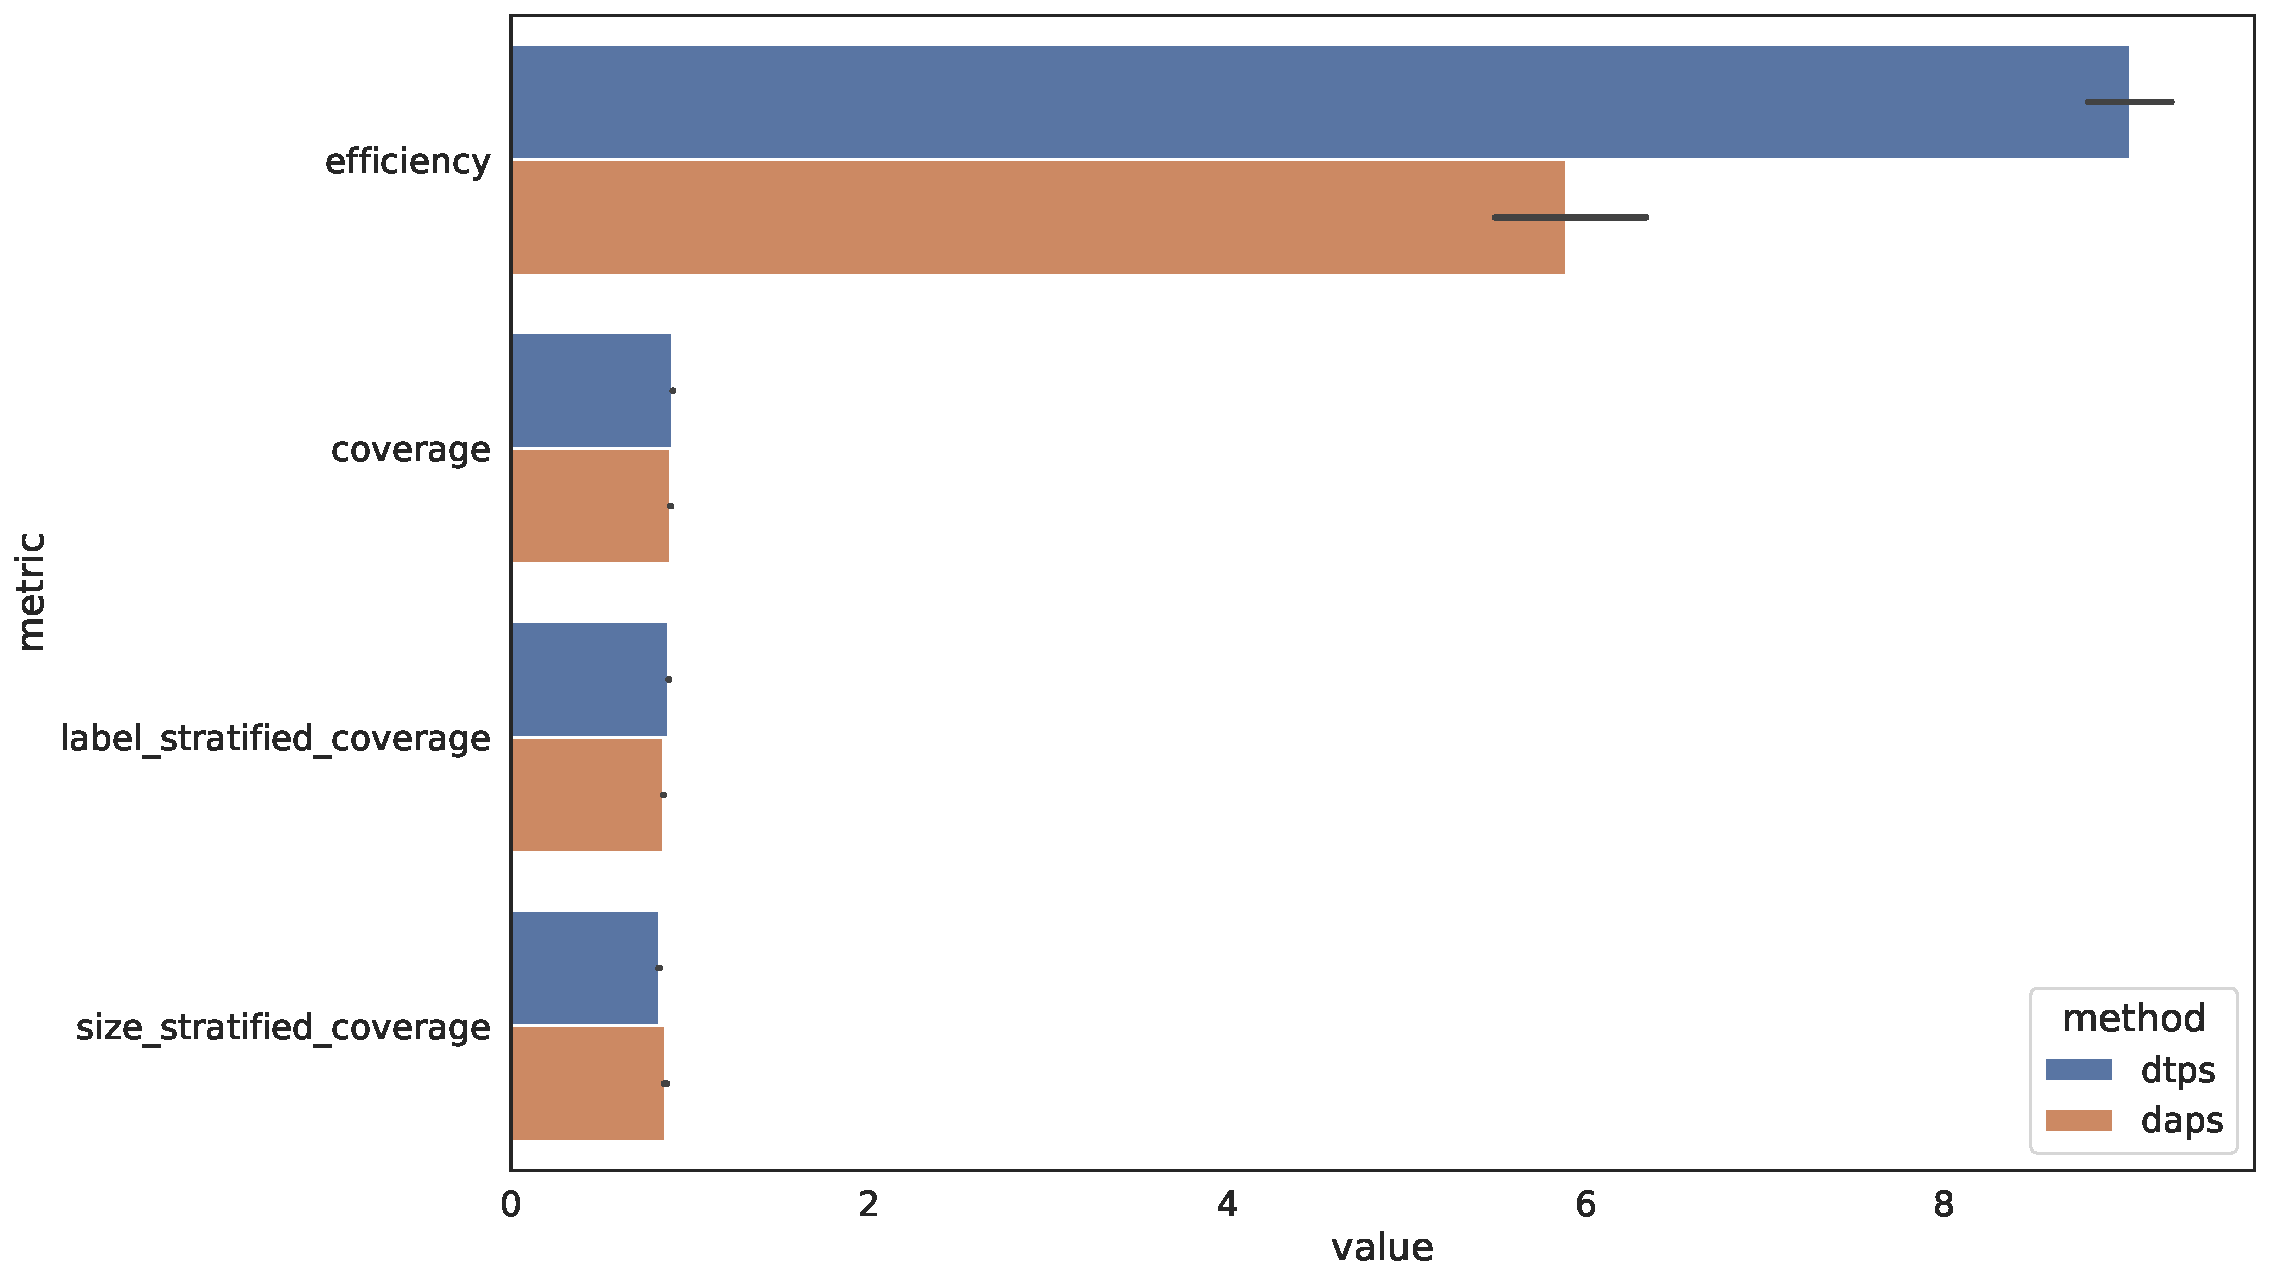
\includegraphics[width=\linewidth]{graphConformal/figures/split/daps_dtps_cora}
    \end{subfigure}
    \caption{Bar charts denoting different metrics associated with DAPS and DTPS across PubMed (top) and Cora (bottom) for the TS split at $\alpha=0.1$. We see that DTPS improves efficiency for PubMed but not for Cora, with minimal impact to other adaptiive metrics.}
    \label{fig:fs:conformal:daps_vs_dtps}
\end{figure}


\begin{figure}
    \centering
    \begin{subfigure}{0.7\linewidth}
        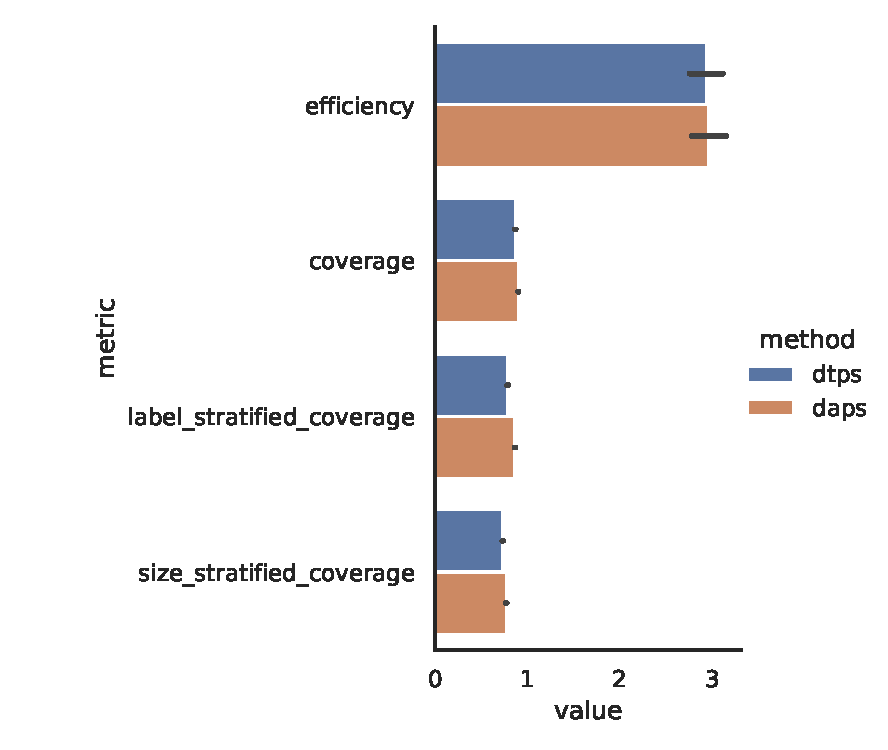
\includegraphics[width=\linewidth]{graphConformal/figures/nspc/daps_dtps_0.1}
    \end{subfigure}
    \begin{subfigure}{0.7\linewidth}
        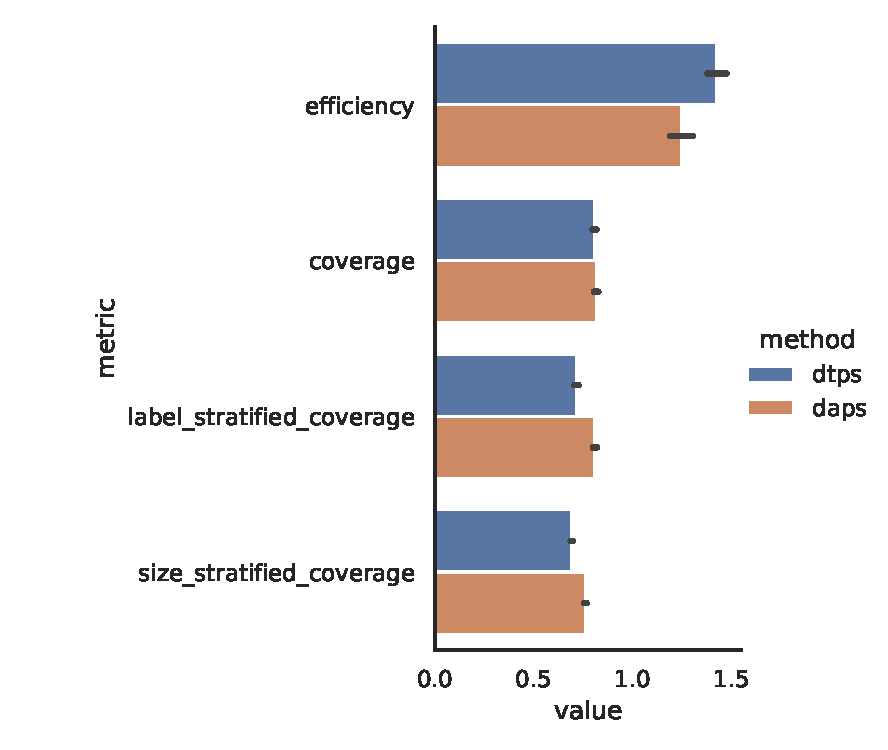
\includegraphics[width=\linewidth]{graphConformal/figures/nspc/daps_dtps_0.2}
    \end{subfigure}
    \caption{Bar charts denoting different metrics associated with DAPS and DTPS across the LC splits at $\alpha=0.1$ (top) and $\alpha=0.2$ (bottom). We see that DTPS deteriorates significantly as compared to DAPS at higher $\alpha$.}
    \label{fig:nspc:conformal:daps_vs_dtps}
\end{figure}

WE compare our proposed Diffusion method--of using TPS-Classwise as the base method--DTPS against DAPS, which was proposed in~\cite{zargarbashi23conformal}.
From Figure~\ref{fig:fs:conformal:daps_vs_dtps}, we see that when the calibration set is large (TS), DTPS can improve efficiency without sacrificing adaptiveness for PubMed but not for Coras.
However, when we control the number of samples per class with LC splits (Figure~\ref{fig:nspc:conformal:daps_vs_dtps}), we see that DTPS deteriorates significantly as compared to DAPS at higher $\alpha$.
Based on these results, we can conclude that DTPS is not a universally better method than DAPS, and its performance is sensitive to the calibration set size and the number of classes.
It may be a viable candidate over DAPS when there is a sufficiently large calibration set.